\documentclass{article}
\usepackage[utf8]{inputenc}
\usepackage{float}

\title{Distributed computing assignment 1: SOA}
\author{t7025t }
\date{}

\usepackage{natbib}
\usepackage{graphicx}

\begin{document}

\maketitle

\section{Services}

\begin{figure}[H]
    \centering
    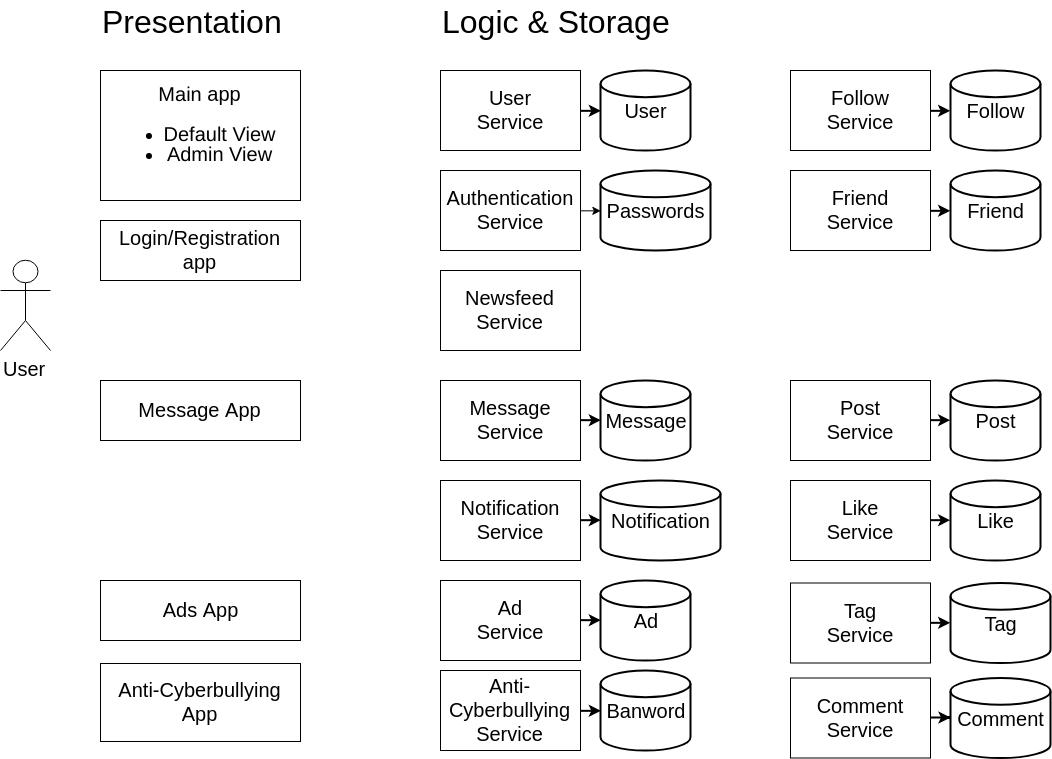
\includegraphics[width=\textwidth]{DC.png}
    \caption{Service oriented architecture}
    \label{soa}
\end{figure}

\begin{description}
    \item [Notification service:] 
    \begin{description}
        \item[]
        \item[In:] POST (notification contents, notification recipient(s) (UID))
        \item[Out:] /
        \item[Logic:] Add notification to DB
        \item[]
        
        \item[In:] GET getnotifications/user\_id 
        \item[Out:] Notifications (ID, Timestamp, Content)
        \item[Logic:] Mark notification as requested
        \item[]
        
        \item[In:] PUT removenotification/notification\_id/user\_id
        \item[Out:] /
        \item[Logic: ] Mark notification as read
    \end{description}
\end{description}



\end{document}
